\documentclass[letter,12pt]{article}
\usepackage{amsmath}
\usepackage{graphicx}
\usepackage{glosstex}
\usepackage[utf8]{inputenc}
\usepackage[spanish]{babel}
\usepackage{tikz,stackengine}

%opening
\title{Reporte 03 Evaluación 07 11 2019}
\author{Eduardo Alexis Valencia Dorantes}
\date{11/Noviembre/2019}
\begin{document}
	
\maketitle{PDF Seno.tex}

\begin{abstract}
Daremos una descripción, paso a paso de como se debe compilar y ejecutar el archivo Seno.tex para poderlo visualizar como documento en PDF.

Omitiremos algunos pasos que ya se dieron en Reporte1.
\end{abstract}

Teniendo en cuenta que el archivo ya fue descargado desde el Classroom de la clase de "Taller de Herramientas Computacionales 2020-I" y ya se encuentra en el directorio de Descargas; debemos abrirlo y revisarlo para que se pueda correr de manera adecuada.

\section*{Abrir el documento}

1 . Ya abierto el documento de LaTex, al compilar el archivo; este no marca error ya que falta que se agregue al archivo un módulo, el cual se llama "listenings".
Entonces lo que debemos hacer es escribir al inicio de nuestro documento como sigue

\begin{figure}[h]
	\centering
e	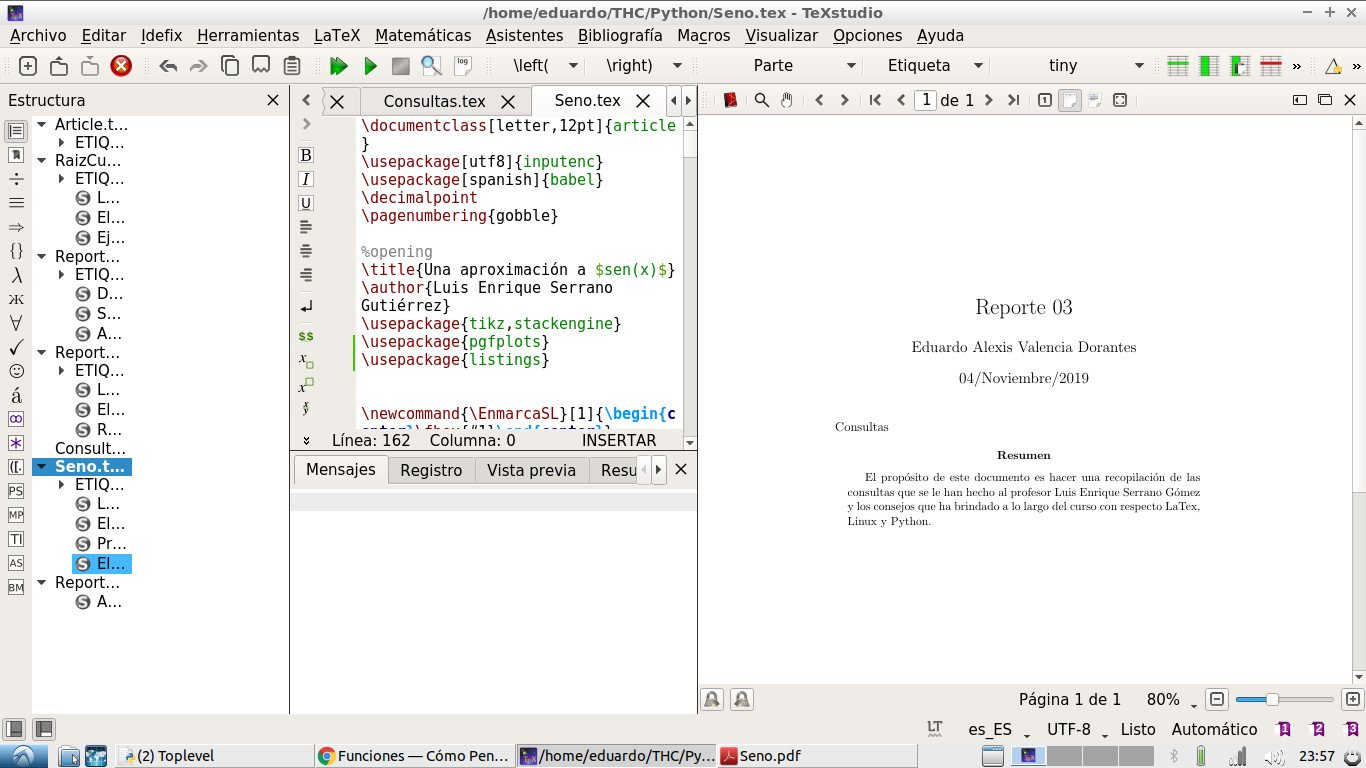
\includegraphics[width=0.7\linewidth]{../../Imagenes/p12.jpg}
	\caption{}
	\label{fig:p12}
\end{figure}

\newpage
2. También debimos haber descargado el archivo de Python que se encuentra de igual forma en el Classroom,y  haberlo guardado en nuestro directorio para que el archivo pueda correr.

3. Teniendo en cuenta ya todo lo anterior, el archivo ya esta listo para visualizarse y abrirse en un PDF.

\begin{figure}[h]
	\centering
	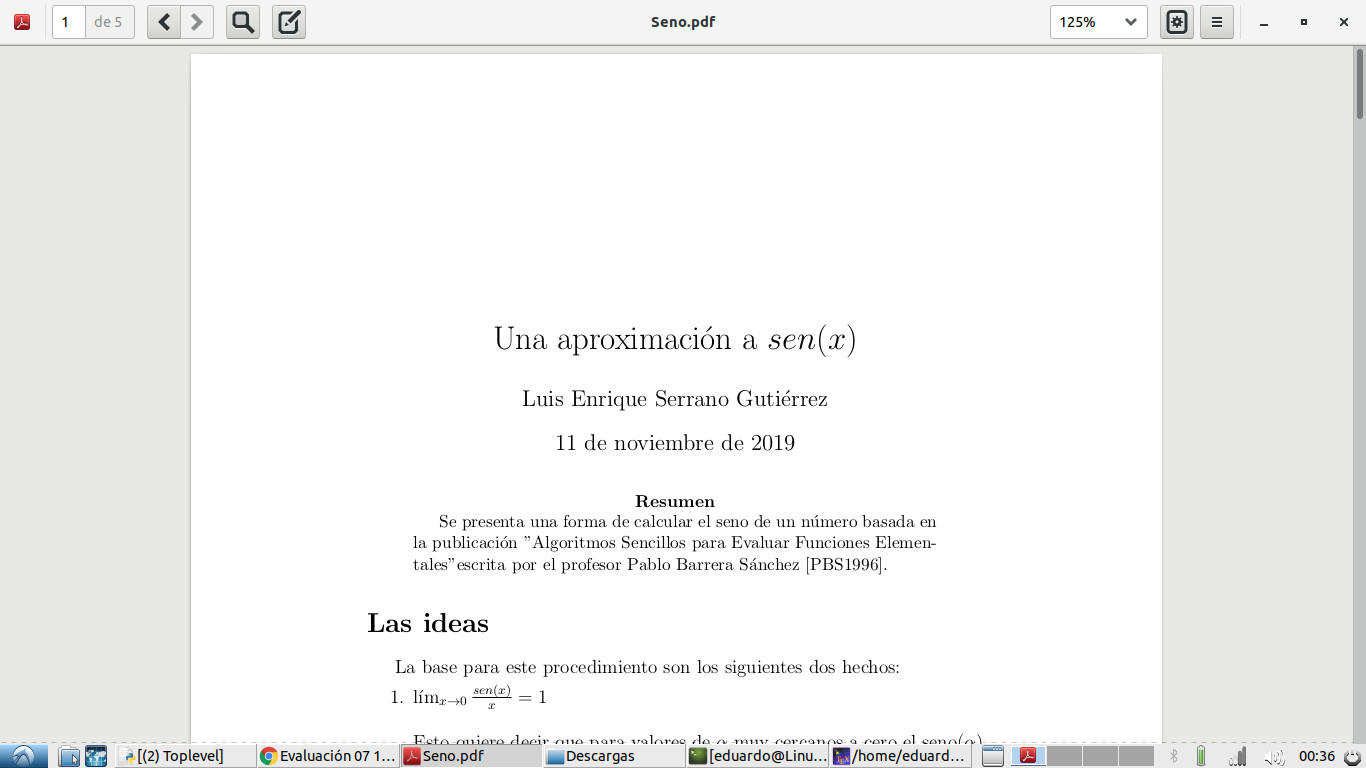
\includegraphics[width=0.7\linewidth]{../../Imagenes/p13.jpg}
	\caption{}
	\label{fig:p13}
\end{figure}





\end{document}